\documentclass[10pt,conference,a4paper]{IEEEtran}

%import packages here
\usepackage{amsmath}
\everymath{\displaystyle}
\usepackage{graphicx}
\usepackage{caption}
\graphicspath{{Images/}}

\title{Internet Attribute Certificate Profile for Authorization (RFC5755) - A Cryptographic Analyses}
\author{Ruud Verbij \\ Student at the University of Twente \\ crypto@ruudverbij.nl}
\begin{document}
\maketitle

\begin{abstract}
This paper touches upon some of the cryptographic and PKI elements concerned with Attribute Certificates. These Attribute Certificates are used to extend the lifetime and functionality of regular Public Key Certificates in a Public Key Infrastructure. The Attribute Certificates are binded to a Public Key Certificate, have a shorter lifetime (quite temporarily) and add attributes from specific services to the Public Key Certificate. The attributes support all sorts of functionality, including authorization, access regulation, charging mechanisms and much more. This paper draws some of the characteristics and usage of Attribute Certificates in a Public Key Infrastructure, aswell as providing the reader with some security requirements when working with them.
\end{abstract}

\begin{IEEEkeywords}
Attribute Certificate, Public Key Infrastructure, RFC5755, PKI, AC, Cryptography
\end{IEEEkeywords}

\section{Introduction}
\label{Introduction}
This paper outlines some of the cryptographic aspects offered by the Attribute Certificates\cite{rfc_ac} to the Public Key Infrastructure as defined by X.509\cite{rfc_x509}. Attribute Certificates (AC) is currently (may 2013) a \texttt{Proposed Standard} with the IETF and is awaiting approval for the \texttt{Draft Standard} category. The RFC5755 which covers AC's will obsolete an old IETF document describing ACs\cite{rfc_oldac}.

The structure of this paper is as follows, Section~\ref{ac_in_pki} will introduce ACs. It covers the role of ACs within the entire PKI, the expected users and their usage of ACs. Section~\ref{cryptography_in_ac} describes what additional security features the use of AC brings and what role cryptography plays. Section~\ref{security_requirements} covers the security requirements involved when using ACs.  

This paper in no way presents a complete overview of the use of ACs within PKI. The reader is referred to \cite{rfc_ac} when working with, or having interest in the use of ACs within a PKI. The author is in no way responsible for any damage caused by this paper. The paper is written for Computer Science experts, especially those with interest in PKI and cryptography. This paper mainly consists of information from the RFC~\cite{rfc_ac}, except for statements which are followed by another reference.

\section{Attribute Certificates in the Public Key Infrastructure}
\label{ac_in_pki}
This section of the paper covers several topics, including an introduction to ACs, examples of usage and the Infrastructure necessary to work with  ACs. The purpose of this section is to describe the role of ACs in the entire picture of PKIs.
\subsection{Introduction to AC}
To begin with, ACs are just like PKI certificates, except for the fact that they lack a public key. This is due to the fact that ACs are not used for any cryptographic purposes, but serve a different role. The main idea of an AC is to bind attributes to the identity of an individual through his/her PKI certificate (PKC). The attributes cover topics like access control, group identity, data origin authentication, etc. They belong to one PKC in the sense that they are mentioned in the AC, more on that in Section~\ref{cryptography_in_ac}.

One may ask \textit{why} we need ACs when we already have PKC, which tend to have more features (a public key ie.). The introduction of ACs actually extends the usability of PKCs. This extention can be split into two different gains:
\begin{itemize}
	\item It provides for a \textit{temporary} set of attributes to be binded to an identity within an organisation. These attributes range from group identities, roles and clearance to charging identities and audit identities. 
	\item ACs allow for the transfer of granting access or authorization, from the general PKC issuer within an organisation to special authorization authorities (AA).
\end{itemize}

ACs are typically used for granting this explicit \textit{temporary} access to a group or a role. This ensures a longer lifetime of the PKC binded to this AC. When the access or role for this individual for the service belonging to the AC is revoked or timed out, the AC is no longer valid, but the PKC can still be used. This is a major advantage to the use of PKCs for this purpose. It furthermore eases the general infrastructure of an organisation in the sense that the AC tells whether the binded identity (PKC) has access to this service instead of an online check for this access. AC' standard also offers the ability of AC revocation, more on that in Section~\ref{security_requirements}.

The RFC~\cite{rfc_ac} compares PKCs to passports and ACs to Visa's. Passports tend to have a longer lifetime than Visa's, and the Visa's are binded to the identity of the owner by their passport. This analogy describes the use of ACs quite good, as Visa's also describe access control. But it lacks some of the extra features ACs offer, which will be described in the next subsection.

 Figure~\ref{fig:diff} shows the differences between an AC and a PKC. As can be seen, ACs hold a value referring to the holder. The RFC~\cite{rfc_ac} prescripes three ways in which such an AC can be bound to a PKC, of which only one may be used per AC.
\begin{itemize}
	\item \texttt{baseCertificateID}, the issuer and serial number of the holder's PKC. \textit{"For any environment where the AC is passed in an authenticated message or session and where the authentication is based on the use of an X.509 PKC, the Holder field SHOULD use the baseCertificateID."}~\cite{rfc_ac}
	\item \texttt{entityName}, the name of the claimant or role. This name must the same as on the PKC.
	\item \texttt{objectDigestInfo}, used to directly authenticate the holder. This objectDigestInfo contains a hash of an object the AC is linked to.
\end{itemize}
Furthermore, it has a value containing the attributes belonging to this AC.

\begin{figure}[h]
	\centering
	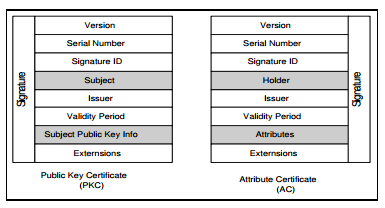
\includegraphics[width=0.5\textwidth]{diff.png}
	\caption{Differences between PKC and AC~\cite{godavari2001secure}}
	\label{fig:diff}
\end{figure}

\subsection{Examples of usage}
An AC can be used in different security related services. \textit{"As an example it could also be used to certify authorization information related to a public key. More specifically, it may be used to limit the liability resulting from a digital signature, or to constrain the usage of a public key (e.g., transaction of a limited value, certain time windows, etc.)."}~\cite{tilborg2011encyclopedia}.

Different default attributes have been proposed, some of which are listed below~\cite{benantar2006access,rfc_ac}.
\begin{itemize}
	\item \texttt{Service Authentication Information}, which identifies the AC holder to the service by name, with optional service-specific authentication information. This attribute could, by using some encryption scheme, also include the holder's identity and password.
	\item \texttt{Charging identity}, which is used to charge the holder for the use of services.
	\item \texttt{Role}, which is used to specify the role the holder has within a specific service.
	\item \texttt{Clearance}, which defines the clearance the holder has for specific information (secret, top-secret, etc.).
	\item \texttt{Group}, which describes the group the holder belongs to.
\end{itemize}

More rough examples~\cite{tilborg2011encyclopedia} indicate the use of ACs for DRM-secured devices. ACs could grant applications the right to install itself on devices like iPads and alike.

\subsection{Public Key Infrastructure to fit AC in}
To use ACs within an organisation, there are mainly two implementation defaults, the so called \texttt{push} and \texttt{pull} models. This paper roughly describes the main arguments for choosing either of the two.

The \texttt{push} model requires the AC holder to own his AC. When speaking to the Server, he/she is required to attach the AC with the request. \textit{"The 'push' model is suitable in application where the client's permissions should be authenticated/validated in the client's 'home' domain."}~\cite{godavari2001secure} This means that no new connections need to be set up between the Server and other parties, as will be in the \texttt{pull} model.

The \texttt{pull} model requires the Server to retrieve the AC from a repository or an AC issuer. This means the implementation does not involve a change in the client-server protocol, which has benefit over the \texttt{push} method when implemented within an existing infrastructure. \textit{"The 'pull' model is suitable when the client's priviliges should be authenticated in the inter-domain"}~\cite{godavari2001secure} Furthermore, there is no need to update client's ACs when they are renewed, this can be done within the repository or AC issuer.

Figure~\ref{fig:PKI_models} shows the different protocol possibilities within one figure. It shows the different possible actors (AC issuer, Client or AC Holder, Server or AC verifier and Repository) and their possible communication flows.

\begin{figure}[h]
	\centering
	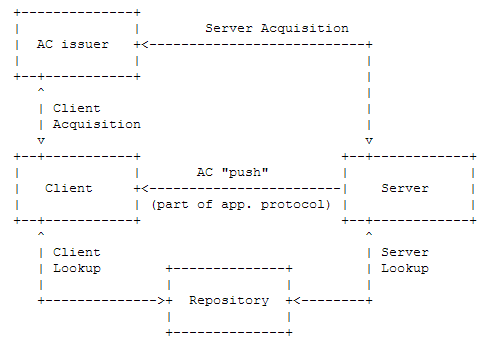
\includegraphics[width=0.5\textwidth]{PKI_models.png}
	\caption{Protocol communication for \textit{push} and \textit{pull} models~\cite{rfc_ac}}
	\label{fig:PKI_models}
\end{figure}

\section{Cryptography in Attribute Certificates}
\label{cryptography_in_ac}
This Section describes the role of cryptography within the use of ACs and the way ACs are constructed and issued by an AC issuer. Lets stress again that this paper is not ment to give a complete overview of the cryptography involved with ACs and the author is in no way responsible for any damage caused by the information in this paper.

\subsection{Issueing of an Attribute Certificate}
Within an organisation, there must be a clear seperation between a Certificate Authority (CA) and an Attribute Certificate Authority (AA) as prescribed by the RFC~\cite{rfc_ac}. Within the same organisation the public key of the AA is distributed and trusted, which means that documents signed by the AA are trusted directly and not via a PKC path. An AA can build an AC and sign it using his private key, which can later on be verified by a Server or Service (AC verifier).

After the AC has been build, either the \texttt{push} or \texttt{pull} model can be used to either distribute the AC to the client, or to distribute it to the AC repository. AC verifiers will verify the validity of an AC for an action or authenticate using the following steps~\cite{rfc_ac}.
\begin{enumerate}
	\item The AC holder's PKC must be present, and the entire certification path of that PKC must be verified.
	\item The AC signature must be cryptographically correct and the issuers PKC certification path must be verified.
	\item The AC issuer must be trusted directly (as mentioned above, the ACs Public Key should be trusted).
	\item The time for which the AC is being evaluated must be within the AC validity.
	\item The AC must follow the standard.
	\item The AC must not contain unsupported critical extensions.
	\item The AC should not have been revoked. (See Section~\ref{security_requirements})
\end{enumerate}

\subsection{Cryptography}
ACs are signed by the AA using a Signature Algorithm which is specified within the AC. The algorithms allowed for the signature are listed in different RFCs~\cite{rfc_alg1,rfc_alg2,rfc_alg3,rfc_alg4}. The RFC~\cite{rfc_ac} states \textit{"The binding between an AC holder and attributes cannot be stronger than the cryptographic module implementation and algorithms used to generate the signature.  Short key lengths or weak hash algorithms will limit the utility of an AC. AC issuers are encouraged to note advances in cryptology so they can employ strong cryptographic techniques."} Which states clear that the responsibility for using proper Signing algorithms lies with the AA.

The other cryptography that could be involved in ACs is the placement of login details (username and password) of an AC owner in the AC itself. In this case, ofcourse measures have to be taken to avoid plaintext passwords in the AC. The RFC~\cite{rfc_ac} let the implementer decide upon proper cryptographic encryption functions necessary for the protection of the login credentials. The RFC~\cite{rfc_ac} suggests the use of Public Key Cryptography (encrypting with the Public Key of the Server or AC verifier). It is again the case that the AA is responsible for good cryptographic management of the issues mentioned previously.

\section{Security Requirements}
\label{security_requirements}
This section discusses the requirements set for the AC (which AC all meets) and discusses the security requirements necessary for securely operating with ACs. Furthermore it will touch upon AC revocation.

\subsection{AC Requirements}
The RFC~\cite{rfc_ac} enumerates a set of requirements they meet with this RFC.
\begin{enumerate}
	\item \textit{"Support for short-lived as well as long-lived ACs. Typical short-lived validity periods might be measured in hours, as opposed to months for PKCs. Short validity periods allow ACs to be useful without a revocation mechanism."} This is met by forceing the use of a validity value on an AC which can be set \texttt{YYYYMMDDHHMMSSZ}.
	\item \textit{"Issuers of ACs should be able to define their own attribute types for use within closed domains."} This is met by allowing attributes to be made by the AAs themselves, though, keeping consistency by forceing the use of some predefined way of defining them.
	\item \textit{"Some standard attribute types, which can be contained within ACs, should be defined. Examples include 'access identity', 'group', 'role', 'clearance', 'audit entity', and 'charging identity'"} This is met by having these implemented as defaults.
	\item \textit{"Standard attribute types should be defined in a manner that permits an AC verifier to distinguish between uses of the same attribute in different domains. For example, the 'Administrators group' as defined by 'Baltimore' and the 'Administrator group' as defined by 'SPYRUS' should be easily distinguished."} This is met by allowing an optional \texttt{roleAuthority} for every \texttt{roleName}.
	\item \textit{"It should be possible to 'target' an AC at one, or a small number of, servers. This means that a trustworthy non-target server will reject the AC for authorization decisions."} This is met by the implementation of so called \texttt{Target} and \texttt{TargetCert} fields.
	\item \textit{"ACs should be defined so that they can either be 'pushed' by the client to the server, or 'pulled' by the server from a repository or other network service, including an online AC issuer."} This is met by the two possible implementation defaults for the Server or AC verifier.
\end{enumerate}

\subsection{Security Requirements for Safe Use}
Several security requirements for safe use of ACs are recommended by the RFC~\cite{rfc_ac}. This subsection discusses most of them. For a complete view of the requirements, the reader is referred to the RFC~\cite{rfc_ac}.

\begin{itemize}
	\item Masquerading of the AA after the private keys have been compromised could lead to serious security problems. The ACs that are created by an attacker are checked offline by a Server or AC verifier, and therefore can cause serious damage. Revocation of the AAs public key (trust in the AA) should be performed to overcome this problems. Detection could be quite hard, since offline verification is possible. This is especially dangerious if the \texttt{push} model is used, in which a rogue client can easily send his rogue AC to the AC verifier.

	\item If an AA loses his private keys, this also leads to serious problems. All revocation lists have to be signed by the AA, and therefore, revocation becomes a critical problem.

	\item AAs are recommended to have an online \texttt{AC Revocation Status Service} by which an AC verifier can easily check the status of an AC. The freshness of the AC Status highly reduces vulnerabilites since these are detected quicker.

	\item Cryptographic hash functions, signing algorithms, public key cryptography, keylengths, etc. all are important since \textit{"The binding between an AC holder and attributes cannot be stronger than the cryptographic module implementation and algorithms used to generate the signature."}~\cite{rfc_ac}.

	\item The RFC~\cite{rfc_ac} is really clear about how and what to check for the binding between the AC and the PKC. An AC verifier should strictly follow the protocol described by the RFC. Not following protocol, especially concering the fields for \texttt{entityName} and \texttt{baseCertificateID} could lead to serious security issues.

	\item It is highly recommended to not use AC chains and to make the signing AA for an AC directly trustworthy.
\end{itemize}

\subsection{AC Revocation}
This paper mentioned AC revocation several times, this subsection will explain the rough base for AC revocation as set by the RFC~\cite{rfc_ac}. Typically, the use of ACs is ment \textit{temporarily}, and therefore revocation should occur less often than one sees within a PKC-like environment. Though, since situations (like some mentioned in the previous subsection) could occur in which revocation is desired, the AC standard allows for mechanisms to revoke ACs. Two mechanisms exist.

The \texttt{Never revoke} scheme MUST be supported by all AC verifiers. This scheme lets ACs contain a possible \texttt{noRevAvail} field, which implicitly means that the status of the AC can be verified at the AA. This particular AC with the \texttt{noRevAvail} field set to true, will never end up on any revocation list and should therefore be checked at the AA.

The \texttt{Pointer in AC} scheme allows for a \textit{pointer} to a revocation list or a source of revocation status information in the AC. The ACs that have fields set to use this scheme can end up at those lists.

It is forbidden for an AC to be in both schemes. If an AC verifier only supports the \texttt{Never revoke} scheme, then all ACs who are using the \texttt{Pointer in AC} scheme must be rejected, since there status cannot be checked online (and the AC verifier does not support the revocation list pointers).

\bibliographystyle{IEEEtran}
\bibliography{IEEEabrv,literature}
\end{document}






























